% --------------------------------------------------------------
% This is all preamble stuff that you don't have to worry about.
% Head down to where it says "Start here"
% --------------------------------------------------------------
 
\documentclass[12pt]{article}
 %%

\usepackage[margin=1in]{geometry} 
\usepackage{amsmath,amsthm,amssymb}
\usepackage{bm}
\usepackage{bbm}
\usepackage{natbib}
\usepackage{booktabs}
\usepackage{graphicx}
\usepackage{subcaption}
\usepackage{caption}
\usepackage{enumitem}
\usepackage{float}
\usepackage[capitalise, noabbrev]{cleveref}
\usepackage{booktabs}
\usepackage{cleveref}
\usepackage{float}


%% tikz
\usepackage{tikz}
\usetikzlibrary{shapes,arrows}

%% macros %%
\newcommand{\N}{\mathbb{N}}
\newcommand{\Z}{\mathbb{Z}}
\newcommand{\calX}{\mathcal{X}} 
\newcommand{\bx}{\textbf{x}}
\newcommand{\bz}{\textbf{z}}
\newcommand{\E}{\text{E}}
\newcommand{\cov}{\text{Cov}}
\newcommand{\var}{\text{Var}}
\newcommand{\pr}{\text{P}}
\newcommand{\diag}{\text{diag}}
\newcommand\indep{\protect\mathpalette{\protect\independenT}{\perp}}
    \def\independenT#1#2{\mathrel{\rlap{$#1#2$}\mkern2mu{#1#2}}}
\newcommand{\dd}{\text{d}}
\newcommand{\secref}[1]{Section \ref{#1}}
\usepackage{tikz}
\usetikzlibrary{shapes, arrows}
%%
\usepackage{wrapfig}
\usepackage{multicol}
\usepackage{amsmath}

%%
\begin{document}


%
% --------------------------------------------------------------
%                            TIKZ
% --------------------------------------------------------------
\usetikzlibrary{arrows.meta,
                chains,
                positioning,
                quotes,
                shapes.geometric}

\tikzset{FlowChart/.style={% this style can be used also at other flowcharts, 
                           % just call it with "FlowChart", see picture code below
startstop/.style = {rectangle, rounded corners, draw, fill=red!30,
                    minimum width=3cm, minimum height=1cm, align=center,
                    on chain, join=by arrow},
  process/.style = {rectangle, draw, fill=orange!30,
                    text width=5cm, minimum height=1cm, align=center,
                    on chain, join=by arrow},
 decision/.style = {diamond, aspect=1.5, draw, fill=green!30,
                    minimum width=3cm, minimum height=1cm, align=center,
                    on chain, join=by arrow},
       io/.style = {trapezium, trapezium stretches body,   % not used in your flowchart
                    trapezium left angle=70, trapezium right angle=110,
                    draw, fill=blue!30,
                    minimum width=3cm, minimum height=1cm,
                    text width =\pgfkeysvalueof{/pgf/minimum width}-2*\pgfkeysvalueof{/pgf/inner xsep},
                    align=center,
                    on chain, join=by arrow},
    arrow/.style = {thick,-Triangle}
                        }
        }% end of tikzset
% --------------------------------------------------------------




% --------------------------------------------------------------
%                         Start here
% --------------------------------------------------------------
%
%\renewcommand{\qedsymbol}{\filledbox}
%
\title{Global Sensitivity Analysis of Stochastic Computer Models with Heteroscedastic GPs}%replace X with the appropriate number
\author{Jack Kennedy} %if necessary, replace with your course title
% 
\maketitle

\section{Intro}

Here we aim to recreate the results of \citet{Marrel2012} using a Gaussian Process (GP) in place of the ``true'' model. Our GP model will be a Bayesian version of HetGP.\\

We aim to compute several sensitivity indices in this report. We will also explain some of the algorithms provided by \citet{Sobol1993}. Our focus here will be to estimate sensitivity indices of the Ishigami function; $f(x) = f(x_1, x_2, x_3) = \sin(x_1) + 7 \sin^2(x_2) + 0.1 x_3^4 \sin(x_1)$. Where each $x_i \in [-\pi, \pi]$. \\

However, the Ishigami function is clearly deterministic, hence we modify it to produce a new function; $f(x, x_\varepsilon) = \sin(x_1) + 7 \sin^2(x_2) + 0.1 x_\varepsilon^2 \sin(x_1)$, with $x_\varepsilon \sim U(-\pi, \pi)$. Although the Ishigami function is simple to compute, in practice we will be working with much more complex systems which will be too expensive for a standard Monte Carlo sensitivity analysis. Hence, we will later replace $f$ by an estimate $\hat{f}$ which will be a GP emulator.\\

Integrating out $x_\varepsilon$ gives us the mean function for our stochastic Ishigami function;

\begin{equation}
	Y_m(x) = \E(Y| x) = \left( 1 + \frac{\pi^4}{50} \right) \sin(x_1) + 7\sin^2(x_2).
\end{equation}

It is also straightforward to find the variance function;

\begin{equation}
	Y_d(x) = \var(Y|x) = \pi^8 (900^{-1} - 2500^{-1}) \sin^2(x_1).
\end{equation}

Notice that $Y_d$ only depends on $x_1$.

\section{Sensitivity Indices \& Their Computation}

\subsection{Sensitivity Indices}

Sensitivity indices allow us to determine how important a group of variable are (or a single variable). They come in two forms, but both are variance based. For a model with $p$ inputs there are $2^p - 1$ such indices, and the sum of all of these indices is exactly one.\\

The first is 

\begin{equation}
	S_i = \frac{\var(Y|X_i)}{\var(Y)}
\end{equation}

which is the proportion of variance that would be eliminated if we were to learn input(s) $i$.\\

The second type is 

\begin{equation}
	S_{T_i} = \sum_{J \supseteq i} S_J 
\end{equation}

which is the total sensitivity to group $i$. For example, in a three parameter problem, the total sensitivity to the first input is

\begin{equation}
	S_{T_1} = S_1 + S_{12} + S_{13} + S_{123}.
\end{equation}

A particularly important index is $S_{T_\varepsilon}$; this is the proportion of uncertainty induced by the random seed variable, including the interaction of the seed variable with the simulator's deterministic components.
\subsection{Computation}

Here we will outline the methods of \citet{Sobol1993} to compute various sensitivity indices for a (stochastic) function $f$. In practice we might replace $f$ by a cheap approximation, $\hat{f}$. We will also have an uncertainty distribution over the inputs. I.e. $x \sim G(x)$, where $G$ is the uncertainty distribution. Further, suppose we can split $x$ into groups $x = (x^1, x^2)$. We can then think about the proportion of variation explained by each group of variables, but a ``group'' might be a single variable (e.g. $x_1$ or $x_\varepsilon$ - uncontrollable variable.\\

We first want to compute the mean value of the mean function, $f_0 = E(Y_m)$
\begin{align*}
f_0 & = \int Y_m(x) \dd G(x) \\
& \approx \frac{1}{N} \sum_{j = 1}^N \hat{Y}_m (x_j)
\end{align*}
where N is a large number, $x_j$ are iid samples from $G(x)$ and $\hat{Y}_m$ is an estimate of the mean function of $f$. When we write $x_j$, we will usually mean a sample from $G(x)$.\\

The variance of $Y_m$ (i.e. the uncertainty in $Y_m$ induced by $G(x)$). This is simply

\begin{align}
	V & = \var(Y_m) \\
	  & = \int Y_m(x)^2 \dd x - f_0^2 \\
	  & \approx \frac{1}{N} \sum_{j = 1}^N \hat{Y}_m(x_j)^2 - f_0^2.
\end{align}

We can find $V_1 = Var(Y | X_1)$ in a similar way:

\begin{align}
	V & = \var(Y_m|X_1) \\
	  & = \int Y_m(x_1)^2 \dd x_1 - f_0^2 \\
	  & \approx \frac{1}{N} \sum_{j = 1}^N \hat{Y}_m(x_1, x_2)\hat{Y}_m(x_1, {x^{2}_j}' ) - f_0^2.
\end{align}
Here, $y_j$ is a draw from $G_1(x^1)$, the marginal distribution of $x^1$, and then $x^2_j, {x^{2}_j}'$ are a pair of independent draws from $G_{2|1}(x^2| x^1 = x^2_j)$

\section{Application to The Ishigami Function}

For the Ishigami function we treat $x_3$ as the random input. Based on a training sample of $500$ data points (no replication) we build a HetGP emulator. We obtain the following estimates for sensitivity measures:

\begin{table}[h]
	\centering
	\begin{tabular}{ccccc}
	\toprule
	& $S_1$ & $S_2$ & $S_{12}$ & $S_{T_3}$ \\ \cmidrule{1-5}
	Exact Values& $0.314$ & $0.442$ & $0$ & $0.244$ \\
	Estimates& $0.318$ & $0.461$ & $0.004$ & $0.228$\\
	$|$Percentage Error$|$& $1.27$ & $4.30$ & $-$ & $6.56$ \\\bottomrule
	\end{tabular}
\end{table}
\section{Conclusions}

We see that $S_{T_3} = S_{T_\varepsilon}$ is estimated to be $0.23$, hence, $23\%$  of output uncertainty is due to the stochastic nature of the simulator. We see $\hat{S}_2 = 0.461$ hence a large proportion of output uncertainty is attributed to $x_2$, similarly, a large (but smaller) proportion of the uncertainty is attributed to the variation in $x_1$. We see that $S_{12}$ is small so it is likely that there is a very weak, or possibly a non-existent, interaction between the two controllable inputs. We also see that the proportion of variance explained by the controllable variables is estimated by $1 - \hat{S}_{T_\varepsilon} = 0.772$, hence the controllable variables dominate the output uncertainty.

\section{Application to Athena model}
\subsection{Sensitivity Indices}
We now apply the above methodology to the Athena model \citep{Zit13, Zit16}. We will use pre-exisiting emulators of the Athena model to perform the computation. We will try a HetGP emulator but also a Stochastic Multilevel (SML) emulator for sensitivity index estimation. Note that the Athena model produces values in the range $[0,1]$, so we in emulate the probit Availability. Hence, sensitivity indices will be for the probit of the output, rather than the output itself.\\

For the distribution over the unknown parameters, we assumed $x_i^* \sim \mathcal{U}(-1.7, 1.7)$ where each $x_i^*$ is the studentised version of the original inputs. Future work would involve producing a distribution over $x$ which is based on Expert opinion.\\

Here we estimate $S_i$ for $i = 1,\ldots,6$ and also $S_{T_\varepsilon}$. The estimates are based on a Monte-Carlo procedure with a sample size of $N = 10^5$.

\begin{table}[h]
	\centering
	\begin{tabular}{cccccccc}
	\toprule
	& $S_1$ & $S_2$ & $S_3$ & $S_4$ &$S_5$ &$S_6$ &$S_{T_3}$ \\ \cmidrule{1-8}
	HetGP& $0.013$ & $0.099$ & $0.039$ & $0.108$ & $0.254$ & $0.151$ & $0.266$ \\
	SML& $0.005$ & $0.080$ & $0.063$ & $0.131$ & $0.285$ & $0.213$  & $0.136$\\ \bottomrule
	\end{tabular}
	\label{Tab:athena-si}
\end{table}

From \Cref{Tab:athena-si} we see that, the (estimated) $S_i$ have the same ordering ($S_5 > S_6 > S_4 > S_2 > S_3 > S_1$). We also see that $S_{T_\varepsilon}^{\text{HetGP}} > S_{T_\varepsilon}^{\text{SML}}$, indicating that the total uncertainty due to the random seed variable is estimated to be larger via HetGP. This could however be larger due to an ill--fitting mean function, and hence deviations from the mean function are being intepreted as noise. \\

The Sobol sensitivity should sum exactly to $1$. In our case we see that $\sum S_i + S_{T_\varepsilon}$ is $0.930$ for HetGP $0.914$ for the SML emulator, suggesting that interactions between the controllable variables are present. The contribution to input uncertainty amongst interaction terms is quite small, but estimated to be slightly larger by SML emulation that HetG.  The total contribution to output uncertainty induced by interactions amongst controllable variables is estimated to be less that $10\%$ in both cases. 

\subsection{Interaction Effects}

We should also investigate which are the largest interactions, should they exist. We, for now, will only do this for the SML emulator.\\

To find the interaction indices, we must first find $V_{ij} = \var \left\{ \E(Y | x_i, x_j) \right\}$. This is the uncertainty induced by the linear and interaction effect between $x_i$ and $x_j$. We then have 
\begin{equation}
S_{ij} = \frac{V_{ij} - V_i - V_j}{\var(Y)}.
\end{equation}

Using a simple Monte-Carlo estimation technique, with $N = 10^5$ samples, we see that the following are the largest interaction terms:

\begin{align*}
	100\hat{S}_{23} = 1.96 \\
	100\hat{S}_{34} = 1.24 \\
	100\hat{S}_{36} = 0.80
\end{align*}

As expected, these interaction effects are quite small. It is interesting to see that all of them have the $3$ in their index - this variable is the cable repair time.
\subsection{Main effect Inference}

Here we aim to  estimate
\begin{equation}
	\E(Y | x_i) = \int _{\mathcal{X}_{-i}} \eta(\bx) \dd G_{-i|i}(X_{-i} | X_i).
\end{equation}

Here, $\E(Y | x_i)$ is the expected response from the simulator if we were to learn the input $X_i = x_i$ (or indeed, this can be generalised if $X_i$ is a group of variables). We compute this for a grid of values over each $i$. In practice, we replace $\eta(\cdot)$ with an emulator (we use the same as constructed earlier). Since the Athena model is stochastic, we replace $\eta(\cdot)$ with an estimate of the simulator mean and use Monte Carlo methods to estimate the integrals. More explicitly, 
\begin{equation}
	\E^* \{ E(Y|x_i)\} \approx \frac{1}{N}\sum_{j=1}^N Y_m(x_{(j)})
\end{equation}

where $x_{(j)}$ are iid draws from $G_{-i|i}(x_i | x_{-i})$
\\

However, we will also want estimates of uncertainty about the expected mean functions. There are two sources of uncertainty in emulators of stochastic functions; the epistemic (extrinsic) uncertainty in the mean and variance due to lack of knowledge of the simulator but also the aleatory (intrinsic) uncertainty due to the stochastic nature of the simulator. Taking the epistemic uncertainty into account will give us an interval for the mean value given $x_i$. Taking both epistemic and aleatory uncertainty into account gives us an interval which represents likely values for a new run of the simulator given $x_i$, as seen below.\\

\begin{figure}
	\centering
	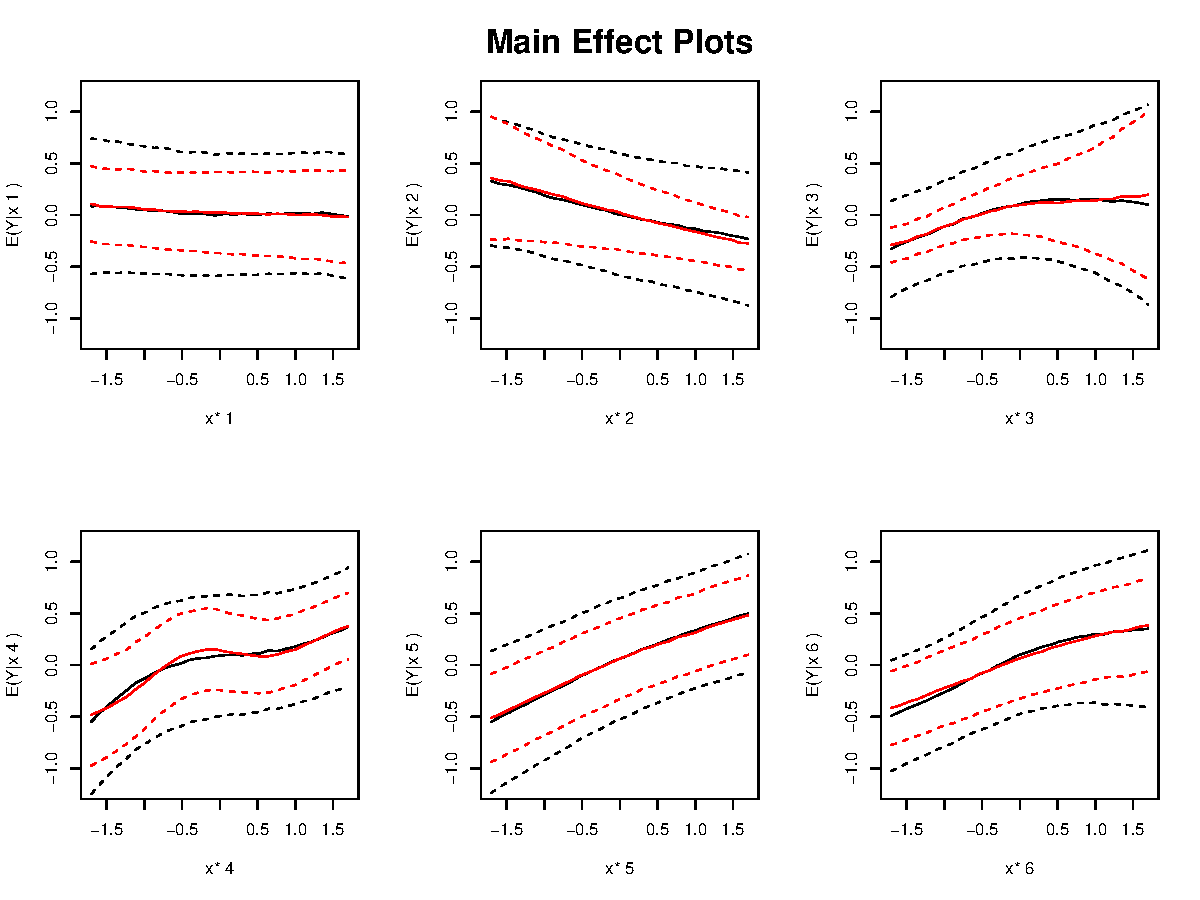
\includegraphics[width = 0.9\textwidth]{fig/main-effects.pdf}
	\caption{Main effect curves (solid) $\pm 2$ standard deviations (dashed). Black represents HetGP and red is SML emulation.}
	\label{Fig:main-effect}
\end{figure}

In \Cref{Fig:main-effect} we see that the effect curves are similar for both HetGP and SML. However, the uncertainty bands are quite different. In this case, the uncertainty bands are calculated in a similar way to the main effects, we integrate the variance over $G_{-i|i}(X_{-i}|X_i)$. Futher, these uncertainty bands represent out ``total'' uncertainty in prediction - they are a combination of the uncertainty in the mean function but also the stochastic nature of the simulator, so give us (approximate) $95\%$ probability bands for a new simulator run, if we were to learn the value of $x_i$. We see that variables $4$ --- $6$ are the most influential, which suggests that the best way to have a windfarm with high availability is to have well functioning components.

\section{Choice of Prior}

To perform the sensitivity analysis, we must specify a distribution, $G$. As mentioned by \cite{Merrel2012}, the model inputs must be deemed as independent in this screening process to ensure a unique ANOVA decomposition of the simulator. We will now perform an investigation into the choice of $G$ subject to a few constraints:\\

\begin{itemize}
	\item Each choice of G has the same mean.
	\item Each choice of G is symmetric.
	\item Each choice of G has a similar $0.05\%$ and $99.5\%$ quantiles.
\end{itemize}

The analysis above used uniform priors over the range of the observed data. However, using a distribution with a hard cut-off may not be satisfactory. For instance, the uncertain input in question could plausibly take any value on the real line, but we just believe that it is likely to be between two limits. We will experiment with a choice of two symmetric, unimodal choice of $G$. First we will try $G(x^*_i) \sim \mathcal{N}(0,0.65^2)$. We will also try $G(X^*_i) \sim 0.536t_{10} $. These were chosen since they give $P(-1.7 < x^*_i < 1.7) = 0.99$. The uniform priors from before have the property $P(-1.7 < x^*_i <1.7) = 1$, so these distributions have similar quantiles. They are also all symmetric, unimodal and have mean $0$. Therefore, each of these priors have many similar summaries. They could all be deemed as an adequate (coarse) representation of beliefs by an expert.\\

We then compute the first order sensitivity idices and $S_{T_\varepsilon}$ via a simple MC method. We can then compare the values of the indices to gauge the relative importance of each variable under different prior specifications.

\begin{table}[ht]
\centering
\begin{tabular}{rrrrrrrr}
  \toprule
 $G$ & $100\hat{S}_1$ & $100\hat{S}_2$ & $100\hat{S}_3$ & $100\hat{S}_4$ & $100\hat{S}_5$ & $100\hat{S}_6$ & $100\hat{S}_{T_\varepsilon}$\\ 
  \cmidrule{1-8}
$\mathcal{U}$ & $0.72$ & $8.18$ & $5.96$ & $13.88$ & $29.17$ & $22.20$ & $13.81$\\ 
  $\mathcal{N}$ & $0.36$ & $7.87$ & $8.56$ & $7.24$ & $25.96$ & $27.12$ & $15.85$\\ 
  $t_{10}$ & $0.50$ & $7.82$ & $9.12$ & $6.28$ & $25.25$ & $28.41$ & $16.96$\\ 
   \bottomrule
\end{tabular}
\caption{Estimated first order sensitivity indices and $S_{T_\varepsilon}$ for three simple choices of $G$.}
\label{Tab:sa-sensitivity}
\end{table}
%% references 


From \Cref{Tab:sa-sensitivity} we see that for the $t_10$ and Normal priors, $S_6 >  S_5 > S_3 > S_2 > S_4 > S_1$ whereas for the uniform prior $S_5 > S_6 > S_4 > S_2 > S_3 > S_1$. The only real agreement between these two formulations is that they both rank $S_1$ as the least informative first order effect. They all rank $S_5$ and $S_6$ as the two most important first order effects. The row sums for the above table are $93.92,$ $92.96$ and $94.34$ respectively (top - bottom). Therefore, in each case the interactions between controllable variables have a similar effect; of the order of $5\% - 7\%$.

\section{Flowchart}


\begin{center}
\resizebox{0.4\textwidth}{!}{
\begin{tikzpicture}[FlowChart,                   % used are styles from tikzset FlowChart
    node distance = 5mm and 7mm,
      start chain = A going below                    % The nodes in the chain
                                                     % will be named by A-1, A-2, ...
                        ]
\node   [process] {Identify uncertain model parameters};               % A-1
\node   [process]   {Identify Experts}; %A-2
\node   [process]   {Perform initial elicitation. Identify a simple, but appropriate, distribution for each parameter.};%A-3
\node   [process]   {Construct emulator.};%A-4
\node   [decision] {Adequate emulator?};%A-5
\node   [process]   {Use sensitivity analysis to identify key inputs.};%A-6
\node   [process]   {Revise the elicitation. Give most attention to the most important inputs.};%A-7
\node   [process]   {Reconstruct emulator in light of refined uncertainty.};%A-8
\node   [decision] {Adequate emulator?};%A-9
\node   [process]   {Compute quanitites of interest.};%A-10
% lines not considered by join macro
\draw [arrow] (A-5.west) to ["no"] ++ (-1.5,0) |- (A-4);
\path   (A-5) to ["yes"] (A-6);
\draw [arrow] (A-9.west) to ["no"] ++ (-1.5,0) |- (A-8);
\path   (A-9) to ["yes"] (A-10);
    \end{tikzpicture}
}
\end{center}


\newpage
\bibliography{/home/b4027030/phd/Writing/references}	%References
\bibliographystyle{agsm}	%BibTeX (.bst) style file
\end{document}
